% --------------------------------------------------------------
% This is all preamble stuff that you don't have to worry about.
% Head down to where it says "Start here"
% --------------------------------------------------------------

\documentclass[12pt]{article}

\usepackage[margin=1in]{geometry}
\usepackage{amsmath,amsthm,amssymb}
\usepackage{graphicx}
\usepackage{subcaption}
\usepackage{algorithmicx}
\usepackage{algorithm}
\usepackage{algpseudocode}
\usepackage[colorlinks,linkcolor=blue]{hyperref}
\usepackage[noabbrev]{cleveref}
\usepackage{courier}
\usepackage{listings}


\oddsidemargin 0in
\evensidemargin 0in
\textwidth 6.5in
\topmargin -0.3in
\textheight 9.0in

\newcommand{\ignore}[1]{}
\def\pp{\par\noindent}

\newcommand{\assignment}[4]{
\thispagestyle{plain}
\newpage
\setcounter{page}{1}
\noindent
\begin{center}
\framebox{ \vbox{ \hbox to 6.28in
{CIS 419/519: Applied Machine Learning \hfill #1}
\vspace{4mm}
\hbox to 6.28in
{\hspace{2.5in}\large\bf\mbox{Homework #2}}
\vspace{4mm}
\hbox to 6.28in
{{\it Handed Out: #3 \hfill Due: #4}}
}}
\end{center}
}

\makeatletter
\renewcommand{\fnum@algorithm}{\fname@algorithm}
\makeatother

\lstset{basicstyle=\footnotesize\ttfamily,breaklines=true}
\lstset{framextopmargin=50pt,frame=bottomline}


\begin{document}

\assignment{Fall 2021}{1}{September 15}{September 27}

% --------------------------------------------------------------
%                         Start here
% --------------------------------------------------------------


{\bf Name: }  QIHANG DAI\\

{\bf PennKey:} ahgdyycc\\

{\bf PennID:} 78803164\\


\section{Multiple Choice \& Written Questions}

\begin{enumerate}
\item
\begin{enumerate}
\item 
\begin{enumerate}
    \item decrease the training error, cause the model is overfitting without regularization on x related value
    \item increase the training error, infinite regularization, underfitting
    \item increase the training error, same as 2
\end{enumerate}
\item
\begin{enumerate}
    \item the intercept can be zero since two class are equal
    \item class 1 have more possibility. $\theta_0$ should be larger so exp(-$\theta_0$) is smaller and the probability is larger
\end{enumerate}
\end{enumerate}

\item
\begin{enumerate}
\item since there is only two point, the boundary should be a perpendicular line to the line connecting two points
\item k =  1, so each data point is its own neighbor, for the dataset each data must have it own label thus the decision boundary is acheived
\item k = infinite, all data points are neighbors, the family would be a constant model that predict all the same output regardless of input 
\item when k is inifinite, the bias is high cause underfitting. when k is 1, the variance is high cause overfit
\item instead of majority vote, we can use square distance, cubic distance, etc. to weight the vote. the higher order of the distance, it gives more weight on the closer points, which increase the true positive rate.  
\end {enumerate}

\item
  \begin{enumerate}
  \item see: \\
        $$P(yes) = \frac{1}{2}$$
        $$H(D) = - \frac{1}{2}log_2(\frac{1}{2}) - \frac{1}{2}log_2(\frac{1}{2}) = 1$$
        $$IG(D, Weather) = 1 - (\frac{3}{8}*(0) + \frac{2}{8} * (0) + \frac{3}{8}(-\frac{1}{3}log_2\frac{1}{3} -\frac{2}{3}log_2\frac{2}{3})) = 0.65 $$
        \begin{flalign} 
        IG(D, WT) &= 1 - (\frac{2}{8}(-\frac{1}{2}log_2\frac{1}{2} -\frac{1}{2}log_2\frac{1}{2}) \\
        & - \frac{3}{8}(-\frac{1}{3}log_2\frac{1}{3} - \frac{2}{3}log_2\frac{2}{3}) \\ 
        & - \frac{3}{8}(-\frac{1}{3}log_2\frac{1}{3} - \frac{2}{3}log_2\frac{2}{3}))\\
        & = \frac{6}{8}(1 - \frac{1}{3}log_2\frac{1}{3} - \frac{2}{3}log_2\frac{2}{3}) = 0.0675
        \end{flalign}
        \begin{flalign} 
          IG(D, Wh) &= 1 - (\frac{3}{8}(0) + \frac{5}{8}(-\frac{1}{5}log_2(\frac{1}{5}) - \frac{4}{5}log_2(\frac{4}{5}))) = 0.55
          \end{flalign}
        thus we choose Weather as the root node to split the data

  \item  pic: \\ 
  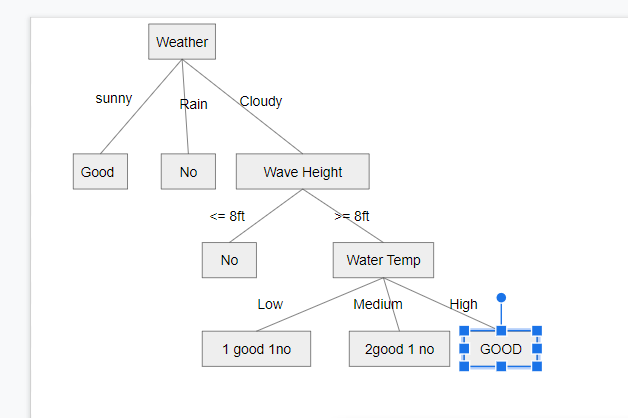
\includegraphics{dt.png}
  \item the probability of be a good day to surf is 2/3, so should be a good day
  \item no. there is error in the leave node as shown in my tree
  \end{enumerate}

\item ans:\\
  For real-valued input, we cant pick a set of thresholds to do binary split. Thus we can calculate different information gain 
  based on different set of thresholds and pick the one with the highest information gain.\\
  For the optimizer, along with the greedily choose the best IG, we can also publish the errorate of the node to gain a better performance, or use Gain ratio to avoid overfitting.\\
\item ans:\\
\begin{gather*} 
  f_{\hat{\beta}}(x) = \hat{\beta}^T x  = x ^ T \hat{\beta} \\
  \hat{\beta} = (X^T X)^{-1} X^T Y \\
  f_{\hat{\beta}}(x) = x^T (X^T X)^{-1} X^T Y \\
  Y = (y1, y2, ..., yn)^T,  \\
  f_{\hat{\beta}}(x) = x^T (X^T X)^{-1} X^T (y1, y2, ..., yn)^T \\
  = \sum_{i=1}^n x^T (X^T X)^{-1} X^T yi \\
  k_i = x^T (X^T X)^{-1} X^T I_i
\end{gather*}
$I_i$ represent (n x 1) vector where only ith element is 1 and others are 0.
 
\end{enumerate}

\section{Python Programming Questions}

% Complete questions in your iPython notebook and place all results here.

TODO: Place your figure and paragraph for Q2.2 here

\vspace{4mm}
\noindent
TODO: Place your figure and paragraph for Q 3.1.2 here

\vspace{4mm}
\noindent
TODO: Place your paragraph for Q3.2 here

\vspace{4mm}
\noindent
TODO: Place your report for Q4.2 here 

\vspace{4mm}
\noindent
TODO: Place your paragraph for Q4.2.1 here 

\vspace{4mm}
\noindent
(if you are attempting 4.3, remember to include your confidence intervals in the performance table)

\end{document} 